%%%%%%%%%%%%%%%%%%%%%%%%%%%%%%%%%%%%%%%%%%%%%%%%%%%%%%%%
\documentclass[12pt,a4paper]{article}% 文档格式
\usepackage{ctex,hyperref}% 输出汉字
\hypersetup{
    colorlinks=true,
    linkcolor=black,
    citecolor=black,
    urlcolor=black
}
\usepackage{fontspec}
\setmainfont{Times New Roman}
%%%%%%%%%%%%%%%%%%%%%%%%%%%%%%%%%%%%%%%%%%%%%%%%%%%%%%%%
\title{\fontsize{26pt}{27pt}\selectfont% 小四字号,1.5倍行距
	{\heiti% 黑体 
	一种基于特征子空间等距线性插值的数据合成方法}}% 题目

\author{\fontsize{15pt}{18pt}\selectfont% 小四字号,1.5倍行距
	{\songti% 仿宋
		郭红建;陆敏;林金官;杜玉坤} 
		% \ thanks{} % 标题栏脚注
		\\
	\fontsize{15pt}{15.75pt}\selectfont% 五号字号,1.5倍行距
	{\songti% 仿宋
		(南京审计大学~~~江苏~南京~~~211815)}}% 作者单位,“~”表示空格
%%%%%%%%%%%%%%%%%%%%%%%%%%%%%%%%%%%%%%%%%%%%%%%%%%%%%%%%
\date{}% 日期(这里避免生成日期)
%%%%%%%%%%%%%%%%%%%%%%%%%%%%%%%%%%%%%%%%%%%%%%%%%%%%%%%%
\usepackage{amsmath,amsfonts,amssymb}% 为公式输入创造条件的宏包
%%%%%%%%%%%%%%%%%%%%%%%%%%%%%%%%%%%%%%%%%%%%%%%%%%%%%%%%
\usepackage{graphicx}% 图片插入宏包
\usepackage{subfigure}% 并排子图
\usepackage{float}% 浮动环境,用于调整图片位置
\usepackage[export]{adjustbox}% 防止过宽的图片
%%%%%%%%%%%%%%%%%%%%%%%%%%%%%%%%%%%%%%%%%%%%%%%%%%%%%%%%
\usepackage{bibentry}
\usepackage[numbers]{natbib}% 以上2个为参考文献宏包
%%%%%%%%%%%%%%%%%%%%%%%%%%%%%%%%%%%%%%%%%%%%%%%%%%%%%%%%
\usepackage{abstract}% 两栏文档,一栏摘要及关键字宏包
\renewcommand{\abstracttextfont}{\heiti}% 摘要内容字体为仿宋
\renewcommand{\abstractname}{\textbf{摘 要}}% 更改摘要二字的样式
%%%%%%%%%%%%%%%%%%%%%%%%%%%%%%%%%%%%%%%%%%%%%%%%%%%%%%%%
\usepackage{url}% 超链接
\usepackage{bm}% 加粗部分公式
\usepackage{amsmath}
\usepackage{multirow}
\usepackage{booktabs}
\usepackage{epstopdf}
\usepackage{epsfig}
\usepackage{longtable}% 长表格
\usepackage{supertabular}% 跨页表格
\usepackage{algorithm}
\usepackage{algorithmic}


\usepackage{changepage}% 换页
%%%%%%%%%%%%%%%%%%%%%%%%%%%%%%%%%%%%%%%%%%%%%%%%%%%%%%%%
\usepackage{enumerate}% 短编号
\usepackage{caption}% 设置标题
\captionsetup[figure]{name=\fontsize{10pt}{15pt}\selectfont 图}% 设置图片编号头
\captionsetup[table]{name=\fontsize{10pt}{15pt}\selectfont 表}% 设置表格编号头
%%%%%%%%%%%%%%%%%%%%%%%%%%%%%%%%%%%%%%%%%%%%%%%%%%%%%%%%
\usepackage{indentfirst}% 中文首行缩进
\usepackage[left=2.50cm,right=2.50cm,top=2.80cm,bottom=2.50cm]{geometry}% 页边距设置
\renewcommand{\baselinestretch}{1.5}% 定义行间距(1.5)
%%%%%%%%%%%%%%%%%%%%%%%%%%%%%%%%%%%%%%%%%%%%%%%%%%%%%%%%
\usepackage{fancyhdr} %设置全文页眉、页脚的格式
\pagestyle{fancy}
\hypersetup{colorlinks=true,linkcolor=black}% 去除引用红框,改变颜色
%%%%%%%%%%%%%%%%%%%%%%%%%%%%%%%%%%%%%%%%%%%%%%%%%%%%%%%%

\begin{document}% 以下为正文内容
%%%%%%%%%%%%%%%%%%%%%%%%%%%%%%%%%%%%%%%%%%%%%%%%%%%%%%%%
	\lhead{}% 页眉左边设为空
	\chead{}% 页眉中间设为空
	\rhead{}% 页眉右边设为空
	\lfoot{}% 页脚左边设为空
	\cfoot{\thepage}% 页脚中间显示页码
	\rfoot{}% 页脚右边设为空
	%%%%%%%%%%%%%%%%%%%%%%%%%%%%%%%%%%%%%%%%%%%%%%%%%%%%%%%%
	\maketitle
	\begin{center}  
		\parbox{\textwidth}{  {\bfseries 摘~~~要:} {\kaishu 考虑到传统噪声处理方法的局限性,本文基于特征子空间插值的思想,提出一种新的处理含噪声数据集的数据合成方法——RELIS(Robust Equidistant Linear Interpolation Synthesis)。
        首先,通过无监督聚类将原始特征空间划分为多个具有近似等量样本的特征子空间;其次,根据聚类结果,引入旅行商问题(TSP)的思想来对特征子空间进行排序;接着,结合软参数共享机制,
        对相邻子空间中的样本进行线性拟合;最后,提出一种创新的多阶段最小权匹配方法来获得较优的插值匹配策略,根据该策略对原始数据集进行等距线性插值。本文从理论上证明了RELIS方法对不同分布的噪声有优化效果,并且在模拟实验
        中验证了该方法的鲁棒性。此外,实验结果表明:RELIS方法还能够显著提升机器学习模型的预测效果。}\\  
		{\bfseries 关键词} {\kaishu 特征子空间;等距线性插值;优化样本;鲁棒性}\\}  
	\end{center}
	\maketitle
	\vbox{\vskip15pt}
	{\Large\textbf{\begin{center}A Data Synthesis Method Based on Equidistant Linear Interpolation in Feature Subspace\end{center}} \par}
	\vspace{1pt}
	\noindent{\bfseries Abstract}\quad 
		In this paper, considering the limitations of traditional noise processing methods, a novel approach for handling noisy datasets based on the concept of feature subspace interpolation is proposed, termed RELIS (Robust Equidistant Linear Interpolation Synthesis).
		First, the original feature space is divided into multiple feature subspaces with approximately equal samples through unsupervised clustering. 
		Second, based on the clustering results, the concept of the Traveling Salesman Problem (TSP) is introduced to order the feature subspaces. 
		Next, by combining a soft parameter sharing mechanism, linear fitting is applied to samples in adjacent subspaces. 
		Finally, an innovative multi-stage minimum weight matching method is proposed to obtain an optimal interpolation matching strategy.
		This paper theoretically demonstrates the optimization effect of the RELIS method for noise of different distributions and further validates it through simulation experiments. 
	\vskip5pt
	\noindent{\bfseries Key words}\quad Feature subspace; linear equidistant interpolation; optimized samples;\\
	\hspace*{2.26cm} robustness 

	\section{引言}
	数据噪声是指数据中任何不准确、不相关或误导性的信息,这些信息可能源于各种原因,例如仪器错误、数据输入错误、传输问题,甚至数据收集过程中的系统偏差 ,是影响数据质量的关键因素之一\cite{bib1}。
	在数据处理和分析的过程中,数据噪声会掩盖真实信息,严重损害统计分析和预测模型的可靠性和准确性。随着数字化转型的进一步推进,实际生活应用中数据体量的不断增加以及数据来源的日趋多样化,
	大数据时代对于数据质量提出了更高的要求,探寻一种能够高效处理含噪声数据集的全新数据合成方法已经成为优化数据质量、提高预测模型准确性和可靠性的关键之举。

	目前已有的数据合成方法包括基于规则、统计、机器学习以及混合等多种形式。这些方法被广泛应用在数据稀缺、隐私保护或模型训练等场景。例如在医疗保健领域,研究人员使用合成数据,
	在确保样本合规性与多样性的同时,可以通过训练模型来提高疾病诊断的准确性和效率,推进医疗科学创新。但现有的数据合成方法对噪声数据集的处理缺乏针对性,例如Chawla\cite{bib2}、Mukhcrjcc\cite{bib3}等人指出SMOTE算法多用于处理不
	平衡数据集,在处理噪声数据方面效果有限; Bond-Taylor\cite{bib4}、Li\cite{bib5}、Creswel\cite{bib6}等人指出GANs等方法则主要学习样本的分布从而产生更多基于该样本分布的数据,并不会从根本上解决数据噪声问题。因此,现有数据合成方法仍面临着对噪声数据的处理不足的挑战。
	
	为了解决处理未知噪声的问题,Chu\cite{bib7}、Lukasik\cite{bib8}、Liguori\cite{bib9}等研究者们提出了多种方法,如数据清洗、数据平滑和异常值检测等。然而,这些方法主要侧重于减轻或消除数据中的噪声,并不能从根本上提升数据质量,存在一定的局限性。
	比如,数据清洗方法难以判断数据噪声和真实的异常值,而某些真实的异常值可能是数据分析中的重要信息源,若在数据清洗的过程中将其视为噪声并移除,可能会导致关键信息的丢失\cite{bib10}。数据平滑技术,如移动平均或高斯平滑,
	虽然可以减少数据中的随机波动,但也可能导致数据过度泛化,这种过度泛化可能会掩盖数据中的重要特征和细节,影响数据分析的准确性 \cite{bib11}。此外,在复杂或更高维度的数据中,噪声和有用信息之间的界限变得更为模糊,数据清理、
	异常值检测\cite{bib12}等降噪方法对于数据集噪声的识别和处理变得更加困难,可能会出现误删大量有价值的数据、保留过多数据噪声等问题。
	在此背景下,本文基于特征子空间线性插值的概念,提出了一种新的数据合成方法,RELIS(Robust Equidistant Linear Interpolation Synthesis)。RELIS可以从两个角度来优化原始数据集。一方面,RELIS方法可以在不丢失
	原始样本信息的情况下合成噪声较小的样本,降低样本的平均误差与高噪声样本的比例;另一方面,RELIS方法可以在特征子空间之间自适应地线性插值样本,增加数据的多样性和代表性,强化了变量之间真实的函数映射关系。相比传统方法,
	RELIS方法更适合机器学习领域的样本噪声处理,即使在处理含有未知复杂噪声的高维数据时,也能有效地增强模型的泛化能力。
	
	本文的内容安排如下:第二节介绍提出的RELIS方法思想及其相关理论;第三节构建了不同的数据集进行数值模拟来验证RELIS的理论性质;第四节将RELIS方法应用到共享单车需求数据;第五节为本文的结论;附录是该方法有效性的证明。

	\section{方法与理论}
	RELIS方法分为四步骤:

	(1).通过无监督聚类算法将原始特征空间划分为多个样本数量几乎相等的子空间。该步骤分为两个阶段,即层次聚类阶段以及K近邻优化阶段;

	(2).随后对子空间之间进行排序,该部分以最小化距离总和为目标将子空间插值排序问题转化为旅行商问题进行求解;

	(3).RELIS方法融合了软参数共享机制的原理,对相邻子空间中的样本进行线性拟合。在这一框架下,虽然每个任务都拥有其独特的模型和权重,但这些任务特定模型的参数之间的差异被纳入到联合目标函数中。这种方法确保局部拟合函数可以考虑全局信息;

	(4).最后,本文提出了一个多阶段最小权匹配算法,该算法可以针对相邻子空间之间的样本快速得到效果较好的插值匹配策略,并根据求得的插值匹配策略对相邻的子空间之间的样本进行多次线性插值。通过特征子空间之间插值合成的样本具有相比原始样本更小的噪音误差,达到扩充数据、优化样本并且强化变量函数关系效果的目的。

	RELIS方法整体流程图如图1所示:


	\begin{figure}[H]% 插入一张图片,H表示浮动环境下的here
		\centering
		\begin{minipage}{0.83\textwidth}% 小页面尺寸,可自行调节
			\centering
			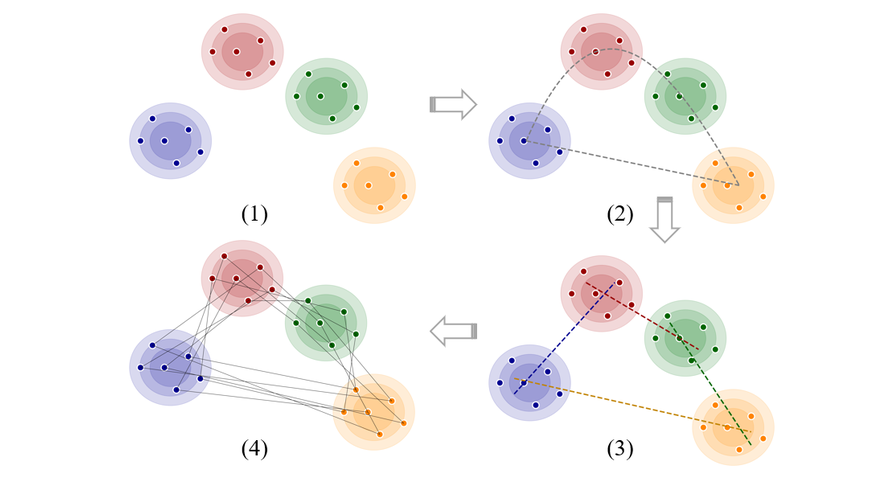
\includegraphics[width=1.0% 图片尺寸,可自行调节
			\textwidth]{流程图.png}% 图片名称(图片需与tex文件在同一文件夹)
			\caption{\fontsize{10pt}{15pt}\selectfont RELIS方法流程图}% 图例
		\end{minipage}
	\end{figure}

	 (1)通过无监督聚类算法将原始特征空间划分为样本量近似相等的多个特征子空间。 (2) 针对二维特征空间的情况解决了 TSP 问题,从而产生子空间插值排序方案。 (3) 在具有相邻排序的子空间之间执行线性拟合。
	 (4)基于线性拟合的结果,通过多阶段最小权重匹配方法得到相邻子空间之间的样本插值匹配策略,并进行插值以合成误差更小的样本。

	\subsection{特征子空间的划分}
	\subsubsection{层次聚类}
	层次聚类的设计主要基于贪心策略,使用无监督算法进行多次迭代聚类,需要先给定初始超参数 $k$,该参数的直观解释为原始特征空间被划分成的子空间的数量。

	在首次迭代阶段,给定一个样本特征的有序集合为$C_1=\left\{\boldsymbol{c}_i \right\}_{i=1}^n=\left\{\boldsymbol{x }_i \right\}_{i=1}^n$,
	其中$\boldsymbol{c}_i$是集合$C_1$中的第$i$个元素。计算得出$C_1$内最接近的一对元素$\boldsymbol{c}_p$ 和 $\boldsymbol{c}_q$,
	$p,q = \underset{\substack{p, q; p \neq q}}{\arg\min} \;\text{dist}(\boldsymbol{c}_p, \boldsymbol{c}_q)$。本文将包含最近两个元素的集合
	$D_{1}=\{\boldsymbol{c}_p,\boldsymbol{c}_q\}$定义为第一个簇,并根据公式 $(1)$计算其簇心:

	\begin{equation} \label{equ1}
		\bar{\boldsymbol{x}}^s = \frac{\sum_{\boldsymbol{x}^s \in D_s} \boldsymbol{x}^s}{\text{num}(D_s)}, 
	\end{equation}
	式$(1)$中 $\text{num}(D_s)$是集合 $D_s$中元素的数量。在首次迭代的最后,把 $\boldsymbol{c}_p$和 $\boldsymbol{c}_q$从集合 $C_1$中删除,并将 $D_1$的簇心添加到 $C_1$作为下一次迭代的初始集合,
	即  $C_{2}=\{\boldsymbol{c}_i \in C_{1} | i \neq p, q\} \cup \{\bar{\boldsymbol{x}}^1\}$。

	在后续迭代中,都需要确定集合 $C_t$中距离最近的两个元素 $\boldsymbol{c}_p$和 $\boldsymbol{c}_q$。对于 $\boldsymbol{c}_p$和 $\boldsymbol{c}_q$需要考虑三种情况:
	$(1)$ 都是原始样本;$(2)$ 一个是样本,一个是簇心;$(3)$ 都是簇心。

	

	当$\boldsymbol{c}_p$和 $\boldsymbol{c}_q$都是原始样本时,将集合 $D_s=\{\boldsymbol{c}_p,\boldsymbol{c}_q\}$定义为一个新的簇,并计算其簇心 $\bar{\boldsymbol{x}}^s$。
	然后,将 $\boldsymbol{c}_p$和 $\boldsymbol{c}_q$从集合 $C_t$中剔除,并将 $\bar{\boldsymbol{x}}^s$添加到 $C_t$中,即 $C_{t+1}=\{\boldsymbol{c}_i \in C_{t} | i \neq p, q\} \cup \{\bar{\boldsymbol{x}}^s\}$。
	
	当 $\boldsymbol{c}_p$是原始样本而 \(\boldsymbol{c}_q:\bar{\boldsymbol{x}}^s\)时,将 $\boldsymbol{c}_p$添加到 $D_s$中,并把 $\boldsymbol{c}_p$从集合 $C_t$中剔除,并根据公式 $(1)$重新计算和更新 $D_s$在 $C_t$中的簇心,
	得到 $C_{t+1}=\{\boldsymbol{c}_i \in C_{t} | i \neq p, q\} \cup \{{\bar{\boldsymbol{x}}^{s\prime}}\}$。

	当 \( \boldsymbol{c}_p:\bar{\boldsymbol{x}}^s, \boldsymbol{c}_q:\bar{\boldsymbol{x}}^l \)时, 合并这两个簇,即$D_s\leftarrow{D_s}{\;\cup\;}{D_l}$,并更新 $D_s$的簇心,
	得到 $C_{t+1}=\{\boldsymbol{c}_i \in C_{t} | i \neq p, q\} \cup \{{\bar{\boldsymbol{x}}^{s\prime}}\}$。

	\begin{figure}[t!]% 插入一张图片,H表示浮动环境下的here
		\centering
		\begin{minipage}{1\textwidth}% 小页面尺寸,可自行调节
			\centering
			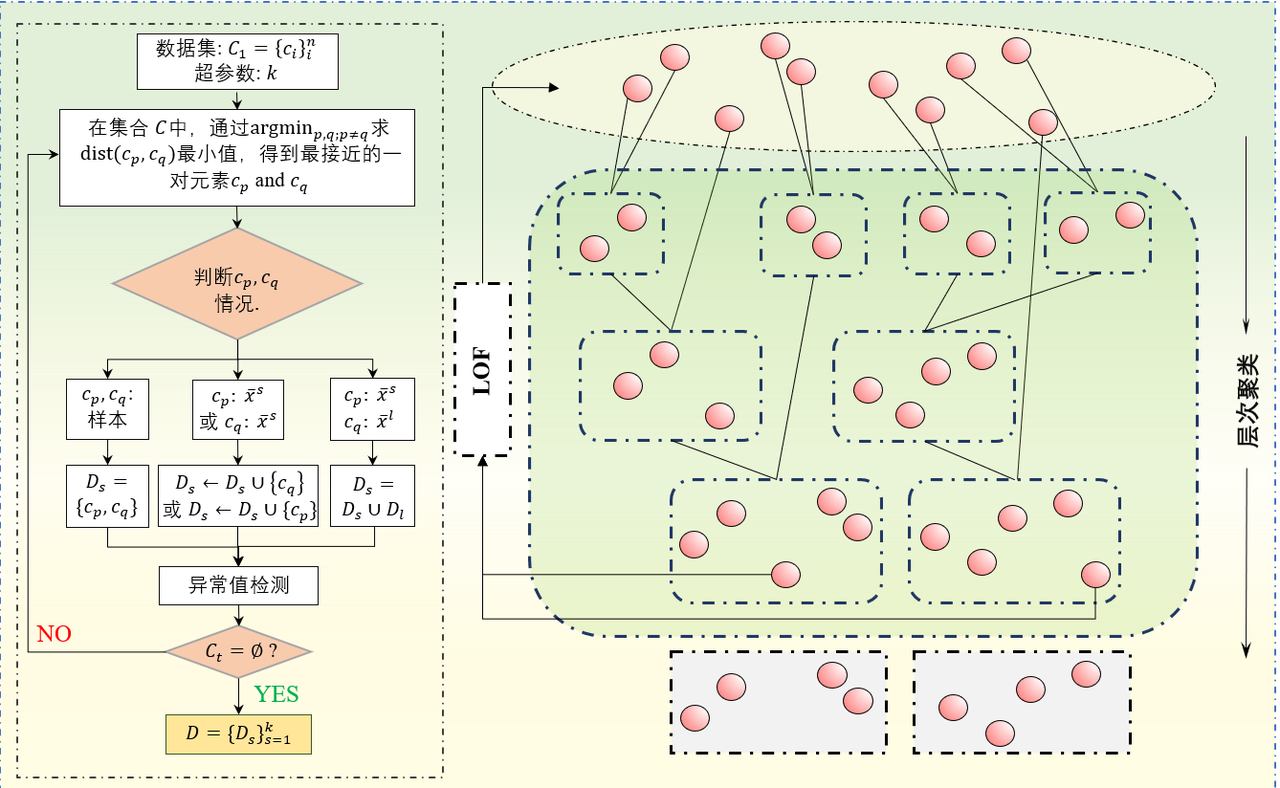
\includegraphics[width=1% 图片尺寸,可自行调节
			\textwidth]{聚类过程.png}% 图片名称(图片需与tex文件在同一文件夹)
			\caption{\fontsize{10pt}{15pt}\selectfont RELIS的层次聚类过程}% 图例
		\end{minipage}
	\end{figure}

	
	% \floatname{algorithm}{算法}
	% \begin{algorithm}[!h]
	% 	\caption{RELIS层次聚类}
	% 	\label{a1}
	% 	\renewcommand{\algorithmicrequire}{\textbf{输入:}}
	% 	\renewcommand{\algorithmicensure}{\textbf{输出:}}
	% 	\begin{algorithmic}[1]
	% 		\REQUIRE 样本特征数据集$C$;超参数$k$  %%input
	% 		\ENSURE $D=\{D_s\}_{s=1}^k$    %%output
	% 		\STATE{当$C\neq{\emptyset}$}
	% 			\STATE{\qquad{}计算得到特征空间中距离最近的两个元素$\boldsymbol{c}_p, \boldsymbol{c}_q$}
	% 			\STATE{\qquad{}分为三种情况进行讨论:}
	% 			\STATE{\qquad{}\qquad{}如果$\boldsymbol{c}_p, \boldsymbol{c}_q$都是样本}
	% 				\STATE{\qquad{}\qquad{}\qquad{}定义新的簇$D_s=\{\boldsymbol{c}_p,\boldsymbol{c}_q\}$}
	% 				\STATE{\qquad{}\qquad{}}\qquad{}计算$D_s$的簇心并添加到集合$C_t$中
	% 				\STATE{\qquad{}\qquad{}\qquad{}将$\boldsymbol{c}_p, \boldsymbol{c}_q$从集合$C_t$中移除}
	% 			\STATE{\qquad{}\qquad{}如果$\boldsymbol{c}_p$是原始样本,\(\boldsymbol{c}_q:\bar{\boldsymbol{x}}^s\)}
	% 				\STATE{\qquad{}\qquad{}\qquad{}$D_s\leftarrow{D_s}\;{\cup}\;\{{\boldsymbol{c}}_q\}$}
	% 				\STATE{\qquad{}\qquad{}\qquad{}在集合$C_t$中更新$D_s$的簇心}
	% 				\STATE{\qquad{}\qquad{}\qquad{}将$\boldsymbol{c}_p$从集合$C_t$中移除}
	% 			\STATE{\qquad{}\qquad{}如果\(\boldsymbol{c}_p:\bar{\boldsymbol{x}}^s\)和\(\boldsymbol{c}_q:\bar{\boldsymbol{x}}^l\)都是簇心}
	% 				\STATE{\qquad{}\qquad{}\qquad{}$D_s\leftarrow{D_s}\;{\cup}\;D_l$}
	% 				\STATE{\qquad{}\qquad{}\qquad{}在集合$C_t$中更新$D_s$的簇心}
	% 				\STATE{\qquad{}\qquad{}\qquad{}将$\boldsymbol{c}_p$,$\boldsymbol{c}_p$从集合$C_t$中移除}
	% 			\STATE{\qquad{}如果$\text{num}(D_s)\;\ge\;\left\lceil n/k\right\rceil$}
	% 				\STATE{\qquad{}\qquad{}将$\bar{\boldsymbol{x}}^s$从集合$C_t$中移除}
	% 				\STATE{\qquad{}\qquad{}利用LOF算法检测并剔除$D_s$中多余的样本}
	% 				\STATE{\qquad{}\qquad{}将$\{\boldsymbol{x}^s_i\}_{i=\left\lceil n/k\right\rceil+1}^{\text{num}(D_s)}$添加至集合$C_t$中}
	% 				\STATE{\qquad{}\qquad{}$D\;\leftarrow\;D\;{\cup}\;D_s$}
	
	% 	\end{algorithmic}
	% \end{algorithm}

	在每次迭代结束时,如果 $\text{num}(D_s){\ge}\left\lceil n/k\right\rceil$,则从 $C_{t+1}$中移除 $\bar{\boldsymbol{x}}^s$。随后,使用LOF算法检测 $D_s$中的离群值,并将多余的样本
	$\{\boldsymbol{x}^s_i\}_{i=\left\lceil n/k\right\rceil+1}^{\text{num}(D_s)}$从 $D_s$中删除。然后,将 $D_s'$视为一个完整的簇不参与后续迭代。最后,将LOF算法\cite{bib14}识别的多余样本重新插入到集合$C_{t+1}$中.
	当 $C_{t+1}= \emptyset $时,停止迭代。迭代聚类的详细流程可以参考图2。

	

	该迭代过程可以将原始数据集划分为 $k-1$个包含相等数量的样本的子集和一个最多包含 $\left\lceil n/k\right\rceil$个样本的额外子集。形式上,本文定义 $D={\cup}^k_{s=1}D_s$, $D_s=\{\boldsymbol{x}_i\}_{i=1}^l$,其中 $1 {\le} l {\le} \left\lceil n/k\right\rceil$。
	此外,RELIS的迭代聚类过程将原始特征空间划分为 $k$个特征子空间,表示为 $\mathcal{X} = \cup_{s=1}^{k} \mathcal{X}^s$。



	\subsubsection{K近邻优化}
	RELIS层次聚类过程基于贪婪策略的思想,这种算法的设计在后期迭代中可能会产生不合理的结果,从而影响整体的聚类效果。因此,本文引入了K近邻(KNN)算法对上
	一阶段得到的聚类结果进行微调和优化。这种优化方法可能会影响每个簇中样本数量的平衡,但它将显著提高聚类的效果。
	
	初始聚类阶段完成后,RELIS的层次聚类阶段为每个样本分配一个标签,表示其所属的簇。在 KNN 优化阶段,会对每个样本计算其在特征空间中的 $\left\lceil n/k\right\rceil$个最近邻的样本。随后,
	更新每个样本的簇标签,以反映近邻样本中最频繁出现的聚类标签。这一过程可能会导致一些样本的簇发生变化,从而引起每个簇内样本数量发生波动。这有可能导致
	样本分布较为分散的簇被吸收至其他簇中,进而消失。然而,此优化过程确保了大多数簇的样本数量保持近似相等,并且显著提升了聚类效果。通过将层次聚类过程与
	KNN优化相结合,可以得到最终的聚类结果 $\{D_s\}_{s=1}^{k'}$,其中 $k'$表示经过KNN优化后簇的数量。这种优化确保了簇间样本数量的均匀性,并且显著提升了聚类的总体质量。
	
	\subsection{子空间插值路径排序}

	通过对原始数据进行聚类可以得到多个子集,每个子集对应不同的特征子空间。RELIS方法是对两个相邻的子空间之间的样本进行插值合成数据,该部分主要针对多个子空间插值路径排序的设计进行分析。
	插值路径的设计思想是从一个子空间出发,经过一次所有的子空间并最终返回到起点,目标是最小化总路径距离。可以转化为旅行商问题 (TSP)进行求解,将该问题表示为加权图的边,路径的距离可以表示为边的权重,设定目标函数为:
	\begin{align}
		\min{\sum\limits_{i=1}^{k'-1}\text{dist}(\boldsymbol{\bar{x}}^i,\boldsymbol{\bar{x}}^{i+1})}+\text{dist}(\boldsymbol{\bar{x}}^{k'},\boldsymbol{\bar{x}}^1). \end{align}
			
	在实际应用中,TSP 被用来解决物流、规划和芯片制造等领域的问题,但是直接解决TSP是非常复杂的,许多研究设计了多种启发式算法和近似算法来找到足够好的解 \cite{bib15,bib16}。虽然这些解不一定是最优的,这些方法通过不同的策略在可接受的时间内寻找到一个近似最短路径。
	为了保证能在可接受的时间内得到足够好的解决方案,首先使用贪婪算法快速找到一个初始解,然后使用3-opt方法对其进行优化并获得最终解 \cite{bib17,bib18}。最终得到一个有序集合$D_\text{sorted}=\{D_{(s)}\}_{s=1}^{k'}$。 
	在本文的后续研究中,将序列相邻的两个子集所对应的子空间定义为相邻的特征子空间。

	\subsection{相邻子空间线性回归拟合}

	给定含噪数据集 $D=\{\boldsymbol{x}_i,y_i\}_{i=1}^n$,其中 $\boldsymbol{x}_i\in \mathcal{X}=\mathbb{R}^d$ ,以及 $y_i\in\mathcal{Y}=\mathbb{R}$。 考虑关系式 $\dot{y}_i=f(\dot{\boldsymbol{x}}_i)$,
	其中 $\dot{\boldsymbol{x}}_i$、 $\dot{y}_i$表示 $\boldsymbol{x}_i$和 $y_i$的去噪真实值。 在RELIS 方法中,假设函数 $f(\cdot)$是连续的,可得:
	\begin{align} \dot{y}_i+\varepsilon_{i,y}=f(\dot{\boldsymbol{x}}_i+\boldsymbol{\varepsilon}_{i,x})+\varepsilon_i, \end{align}
	其中 $\boldsymbol{\varepsilon}_{ix}$和 $\varepsilon_{i,y}$分别表示 $\dot{\boldsymbol{x}}_i$和 $\dot{y}_i$中包含的噪声 , $\varepsilon_i$ 是等式的误差项。 等式 $(3)$可以转化为:
	\begin{align} y_i=f(\boldsymbol{x}_i)+\varepsilon_i. \end{align}
	
	通过上述聚类以及排序方法,原始数据集$D$可以划分为多个有序子集 $D_\text{sorted}=\{D_{(s)}\}_{s=1}^{k'}$,其中$D_{(s)}=\{ \boldsymbol{x}_i^s,y_i^s \}_{i=1}^{\text{num}(D_{(s)})}$,
	并且特征空间可以划分为多个有序的子空间 $\mathcal{X}=\cup_{s=1}^{k^\prime}\mathcal{X}_{(s)}$。 对于两个相邻的特征子空间,由于假设函数$f(\cdot)$是连续的,函数$f(\cdot)$ 可以被近似拟合为线性函数 $g(\cdot)$,
	因此等式$(4)$可以转化为:
	\begin{align} y_i^{s,s+1}=g_{s,s+1}(\boldsymbol{x}_i^{s,s+1})+\varepsilon_i+\varepsilon_i^\prime, \end{align}
	其中,$g_{s,s+1}(\cdot)$和 $\varepsilon_i^\prime$分别表示相邻特征子空间$\mathcal{X}^{(s)}$和$\mathcal{X}^{(s+1)}$中的线性拟合函数以及线性拟合误差, 
	$\{\boldsymbol{x}_i^{s,s+1},y_i^{s,s+1}\}\in D_s\cup D_{s+1}$。如果两个子空间之间的距离足够近并且测度趋于0,则线性拟合误差 $\varepsilon_i^\prime\rightarrow0$。

	对相邻的两个子空间进行线性拟合,可以考虑使用普通最小二乘法 (OLS)、Lasso 回归或局部加权线性回归等方法\cite{bib19,bib20,bib21}。 然而,在假设$f(\cdot) $是连续函数的前提下,仅基于两个子空间的样本进行线性拟合并不能充分考虑全局信息。
	因此,本文引入了软参数共享机制\cite{bib22,bib23,bib24},同时估计多个子空间之间的线性拟合函数,并在损失函数中添加了$L_1$正则化项。 这种方法确保每个线性函数 $\hat{g}_{s,s+1}(\cdot)$的估计都融入了全局信息:
	\begin{equation} \label{equ8}
		\begin{aligned}
			L(\boldsymbol{\beta}) = & \sum\limits_{s=2}^{k^\prime-1}\left(L_2(\boldsymbol{\beta}^{s,s+1}) + \frac{\lambda}{\text{dist}(\overline{\boldsymbol{x}}^{s}, \overline{\boldsymbol{x}}^{s-1}) + 1}L_1(\boldsymbol{\beta}^{s,s+1}, \boldsymbol{\beta}^{s-1,s}) \right) \\
			&+ \frac{\lambda}{\text{dist}(\overline{\boldsymbol{x}}^{k^\prime}, \overline{\boldsymbol{x}}^{1}) + 1}(L_1(\boldsymbol{\beta}^{1,2}, \boldsymbol{\beta}^{k^\prime,1})+L_1(\boldsymbol{\beta}^{k^\prime,1},
			\boldsymbol{\beta}^{k^\prime-1,k^\prime}))\\
			& + L_2(\boldsymbol{\beta}^{1,2}) + L_2(\boldsymbol{\beta}^{k^\prime,1}),
		\end{aligned}
	\end{equation}
	其中,
	$$\boldsymbol{\beta}=\left(\boldsymbol{\beta}^{1,2},\boldsymbol{\beta}^{2,3},\ldots,\boldsymbol{\beta}^{k^\prime-1,k^\prime},\boldsymbol{\beta}^{k^\prime,1}\right)^\prime,$$ 
	$$L_2(\boldsymbol{\beta}^{p,q})=\left\|\boldsymbol{y}^{p, q}-\boldsymbol{X}^{p, q} \boldsymbol{\beta}^{p, q}\right\|_{2}^{2},$$ 
	$$L_1(\boldsymbol{\beta}^{q,r},\boldsymbol{\beta}^{p,q})=\|\boldsymbol{\beta}^{q,r}-\boldsymbol{\beta}^{p,q}\|_1,$$ 
	$\dfrac{\lambda}{\text{dist}(\overline{\boldsymbol{x}}^{s},\overline{\boldsymbol{x}}^{s-1})+1}$用作正则项的参数,可以自适应的根据子空间之间的距离进行调整。 在后文实验中,将 $\lambda$设置为1。可以明显看出,公式(6)是一个凸函数,这确保了该函数局部最优解就是全局最优解。
	\subsection{多阶段最小权匹配}
	
	接下来需要对相邻的两个子空间的样本进行等距线性插值合成新的样本,插值的过程是在两个样本之中进行的。RELIS方法生成的数据要充分考虑到所有的样本信息,插值规则如下:
	
	(1). 用于线性插值的两个样本应来自不同且相邻的子空间。

	(2). 每个样本必须至少参与插值过程一次。

	(3). 插值总共将执行 $\max(\text{num}{(D_{(s)}),\text{num}(D_{(s+1)})})$次。

	(4). 所有样本参与插值的次数必须一致。 具体来说,允许每个样本参与插值过程最多$\left\lceil \frac{\max(\text{num}{(D_{(s)}),\text{num}(D_{( s+1)})})}{\min(\text{num}{(D_{(s)}),\text{num}(D_{(s+1)})})}\right\rceil $次。
	
	由于数据集 $D_{\text{sorted}}$包含未知噪声,插值合成的样本受到原始样本噪声的影响也会包含噪声。在两个相邻子空间之间进行插值时,插值匹配策略的选择需要考虑到合成样本相比真实分布的误差。
	不失一般性,假设 $\text{num}(D_{(s)})=m, \text{num}(D_{(s+1)})=n$, 且$n /2\le m \le n$。根据插值规则,共有 $C_{n-2k}^{2}\prod_{k=0}^{n-m-1} C_{m}^{n-m}(2m-n)!$种不同的插值匹配策略可供选择。
	如何快速选择一个较优的插值匹配策略是本文需要重点探讨的问题。
	
	同样不失一般性,假设特征空间的维度是一维的。 用公式$(7)$来量化两个原始样本之间进行线性等距插值合成的样本的平均误差:
	\begin{align} \bar{S}(x^s,x^{s+1})=\frac{\int_{x^s}^{x^{s+1}}|f(x)-l(x)|  dx}{|x^{s+1}-x^s|}, \end{align}
	 $l(x)$表示通过点 $(x^s,y^s)$和 $(x^{s+1},y^{s+1})$的线性函数,$f(\cdot)$代为$x$和$y$的真实函数关系。

	\textbf{定理 1.} 对于两个相邻子空间 $\mathcal{X}_{(s)}$和$\mathcal{X}_{(s+1)}$,考虑到$(x^s,y^s)\in D_{(s)}\ $和$(x^{s+1},y^{s+1})\in D_{(s+1)}$,其中$y=f(x)+\varepsilon$。 根据式(7),假设线性拟合误差 $\varepsilon^\prime\rightarrow0$,可得: 
	
	\begin{align}
		\mathbb{E} (\bar{S}(x^s,x^{s+1}))< \mathbb{E}(\frac{|\varepsilon^s|+|\varepsilon^{s+1}|}{2}).
		\end{align}

		根据定理1,在线性拟合误差 $\varepsilon_i^\prime\rightarrow0 $的假设下,即使在面对噪声不同分布的情况下,对任意两个子空间的样本进行等距线性插值生成的样本均匀噪声的期望小于原始样本噪声的平均期望。

	\textbf{定理 2.} 基于定理 1 ,设 $y^s=f(x^s)+\varepsilon^s$, $y^{s+1}=f(x^{s+1 })+\varepsilon^{s+1}$。 假设线性拟合误差 $\varepsilon^\prime\rightarrow0$, 可得:
	\begin{align}
		\bar{
		S}(x^s,x^{s+1})= \begin{cases} 
		\dfrac{|\frac{\varepsilon^s}{\varepsilon^s-\varepsilon^{s+1}}|\cdot |\varepsilon^{s}|+|\frac{\varepsilon^{s+1}}{\varepsilon^s-\varepsilon^{s+1}}|\cdot|\varepsilon^{s+1}|}{2},\quad\varepsilon^s\cdot \varepsilon^{s+1}<0,
		\\
		\\
		\dfrac{|\varepsilon^s|+|\varepsilon^{s+1}|}{2}, \qquad\qquad\qquad\qquad\quad\varepsilon^s\cdot \varepsilon^{s+1}\ge0.
		\end{cases}
		\end{align}
		
		根据定理 2,式 $(7)$可以转化为式 $(9)$。 我们可以利用子空间之间的线性拟合函数来估计样本误差,然后利用二分图最小权匹配的方法,根据误差信息确定匹配策略。在假设条件下,样本的噪声可以由式$(5)$得到:
		\begin{align} 
			\varepsilon_i^{s,s+1}=y_i^{s,s+1}-g_{s,s+1}(\boldsymbol{x}_i^{s,s+1})
			\end{align} 
	

		根据插值规则,要求每个样本至少进行一次插值,并且约束了插值的总次数。 经过K近邻优化后,子空间之间的样本数量大多数情况并不是完全相等的,所以这不能视作一个最小权完美匹配问题。
		这个问题是一个加权匹配问题的变体,同时融合了平衡匹配和最小权匹配的特点,因为它需要最小化匹配的总权重,并且约束了样本匹配次数的均匀性。
		目前针对这种问题并没有一个现成的标准算法,因此需要对传统的最小权匹配问题进行改进以适应此目标场景。基于此,本文提出了一种启发式的多阶段最小权重匹配方法对该问题进行分析。
		需要注意的是,该方法并不能保证所得的结果是一个最优解,但它可以在极短的时间内得到一个合理的近似解。

		根据上文的假设, $\text{num}(D_{(s)})=m, \text{num}(D_{(s+1)})=n, n/2\le m\le n$。 在这种情况下, $D_{(s)}$中的每个样本都需要进行一次或者两次的插值,并因此将该问题分为两个阶段进行求解。 
		
		给定一个加权二分图  $G=(D_{(s)},D_{(s+1)},E)$,其权重函数为 $\omega:E\rightarrow\mathbb{R}$ ,其中 $D_{(s)},D_{(s+1)}$是两边的顶点集, $E\subseteq D_{(s)}\times D_{(s+1) }$为边集。 
		根据公式 $(9)$,令权重函数 $\omega(\boldsymbol{x}^{s},\boldsymbol{x}^{s+1})=\bar{S}(\boldsymbol{x}^{s},\boldsymbol{x}^{s+1})$。 考虑目标函数: 
		$$\begin{aligned}
			&\quad\;\text{min}\textstyle\sum\limits_{(i,j)\in{E}}\omega(\boldsymbol{x}^{s}_i,\boldsymbol{x}_j^{s+1})v_{i,j},\\
			&s.t.\; \textstyle\sum\limits_{i=1}^{m}v_{i,j}\in{1,2},\forall j\\  
			&\quad\;\;
			\textstyle\sum\limits_{j=1}^nv_{i,j}=1,\forall i
			\end{aligned}$$
		其中 $v_{i,j}$ 是0-1决策变量。

		\floatname{algorithm}{算法}
		\begin{algorithm}[b!]
			\caption{多阶段最小权匹配}
			\label{a2}
			\renewcommand{\algorithmicrequire}{\textbf{输入:}}
			\renewcommand{\algorithmicensure}{\textbf{输出:}}
			\begin{algorithmic}[1]
				\REQUIRE $D_{(s)}=\{\boldsymbol{x}_i^{s},y_i^s\}_{i=1}^m;\;D_{(s+1)}=\{\boldsymbol{x}_i^{s+1},y_i^{s+1}\}_{i=1}^n(m\le{n});\;\hat{g}_{s,s+1}$  %%input
				\ENSURE 插值匹配策略$M$    %%output
				\STATE{根据公式$(10)$估计$D_{(s)} \;\text{和}\;D_{(s+1)}$}中样本的噪音
				\STATE{定义二分图$G_1=(D_{(s)},D_{(s+1)},E)$以及权重函数$\omega(\boldsymbol{x}^{s},\boldsymbol{x}^{s+1})=\bar{S}(\boldsymbol{x}^{s},\boldsymbol{x}^{s+1})$}
				\STATE{当$t=1,2,\ldots,\left\lceil\frac{n}{m}\right\rceil$时:}
					\STATE{\qquad{}使用匈牙利算法求解二分图$G_t$,得到最大匹配$M_t$}
					\STATE{\qquad{}定义$M_t$中参与匹配的顶点集$D_{\text{matched}}\subset{D_{(s+1)}}$}
					\STATE{\qquad{}$D'_{(s+1)}\leftarrow D_{(s+1)}-D_{\text{matched}}$}
					\STATE{\qquad{}定义$G_{t+1}=(D_{(s)},D'_{(s+1)},E')$,其中$E'\subseteq D_{(s)}\times D'_{(s+1)}$}
					\STATE{\qquad{}$M\leftarrow{M}\cup{M_t}$}
			\end{algorithmic}
		\end{algorithm}

		第一阶段中,在不考虑任何约束的情况下,使用匈牙利算法对二分图 $G$求解得到最大匹配 $M_1$。此时 ,每个顶点 $\boldsymbol{x}^s\in D_{(s)}$ 被匹配一次, $D_{(s+1)}$中的 $m$ 顶点也匹配一次, 
		$D_{(s+1)}$中剩余的 $n-m$顶点还未参与匹配,将未匹配的顶点定义为$D'_{(s+1)}$。

		第二阶段中,定义二分图 $G'=(D_{(s)},D'_{(s+1)},E')$,其中 $E'\subseteq D_{(s)}\times D'_{(s+1)}$。使用匈牙利算法对 $G'$求解得到最大匹配 $M_2$。
		由于 $n/2\le m\le n$, $D'_{(s+1)}$中的每个顶点都参与 $M_2$中的一次匹配,而 $D_{(s)}$中的 $m-n$个顶点再次参与了一次匹配。 最终匹配策略 $M=M_1\cup{M_2}$。

		上述是针对二阶段最小权匹配的场景,如果两个子空间之间的样本数量差距较大,则需要分为 $\left\lceil \frac{\max(\text{num}{(D_{(s)}),\text{num}(D_{(s+1)})})}{\min(\text{num}{(D_{(s)}),\text{num}(D_{(s+1)})})}\right\rceil$个阶段处理,更一般的描述见算法1。


	\subsection{RELIS总体分析}

	经过RELIS方法的层次聚类以及$KNN$优化后,原始特征空间被划分为 $k'$个子空间,因此需要进行 $k^\prime$次多阶段最小权匹配以获得 $k^\prime$个匹配策略。根据所有的插值匹配策略,
	可以得到所有样本之间插值路径的总距离,记为 $\text{dist}_{\text{sum}}$。给定一个额外的超参数 $\eta$,该超参数直观的解释是合成样本数量与原始样本数量的比率,该超参数可以自适应控制合成样本的数量。

	对于两个来自相邻子空间中的样本 $\{\boldsymbol{x}^s,y^s\}$ 和 $\{\boldsymbol{x}^{s+1},y^{s+1}\}$,本文定义合成的样本为\\
	$\{\boldsymbol{x}_{(d)}^{s,s+1},y_{(d)}^{s,s+1} \}_{d=1}^{\left\lceil \frac{n\eta }{\text{dist}_{\text{sum}}}\text{dist}(\boldsymbol{x}^s,\boldsymbol{x}^{s+1})\right\rceil}$,
	其中 $n$是原始样本数量,$\dfrac{n\eta}{\text{dist}_{\text{sum}}}$是单位距离插入样本的数量,合成样本的总数量为$\left\lceil \dfrac{n\eta}{\text{dist}_{\text{sum}}}\text{dist}(\boldsymbol{x}^s,\boldsymbol{x}^{s+1})\right\rceil$。

	假设所有变量都是连续的,则线性插值公式如下:

	\begin{align}
		\boldsymbol{x}^{s,s+1}_{(d)}=\boldsymbol{x}^s+d\dfrac{\boldsymbol{x}^{s+1}-\boldsymbol{x}^{s}}{\left\lceil \frac{n\eta}{\text{dist}_{\text{sum}}}\text{dist}(\boldsymbol{x}^s,\boldsymbol{x}^{s+1})\right\rceil+1},
		\end{align}

	\begin{align}
		y^{s,s+1}_{(d)}=y^s+d\dfrac{y^{s+1}-y^{s}}{\left\lceil \frac{n\eta}{\text{dist}_{\text{sum}}}\text{dist}(\boldsymbol{x}^s,\boldsymbol{x}^{s+1})\right\rceil+1}.
		\end{align}

		\begin{algorithm}[t!]
			\caption{RELIS方法}
			\label{a3}
			\renewcommand{\algorithmicrequire}{\textbf{输入:}}
			\renewcommand{\algorithmicensure}{\textbf{输出:}}
			\begin{algorithmic}[1]
				\REQUIRE 原始数据集$D=\{\boldsymbol{x}_i,y_i \}_{i=1}^n$;超参数$k$,$\eta$
				\ENSURE 优化后的数据集$D^\prime$
				\STATE{构建特征数据集$C=\{\boldsymbol{x}_i\}_{i=1}^n$}
				\STATE{对集合$C$进行层次聚类以及KNN优化,可得聚类结果$D=\{D_s\}_{s=1}^{k^\prime}$}
				\STATE{构建加权图,使用贪心算法求解插值路径初始排序解}
				\STATE{使用3-opt算法优化初始解,得到排序好的插值路径$D_{\text{sorted}}=\{D_{(s)}\}_{s=1}^{k^\prime}$。}
				\STATE{对子空间之间进行线性拟合得到$\{\hat{g}_{s,s+1}\}_{s=1}^{k^\prime-1}\cup\{\hat{g}_{k^\prime,1}\}$}
				\STATE{对于$s=1,2,\ldots,k'$,执行以下步骤:}
					\STATE{\qquad{}对数据集$D_{(s)},D_{{(s+1)}}$估计样本噪音$\varepsilon_i^{s,s+1}=y_i^{s,s+1}-\hat{g}_{s,s+1}(\boldsymbol{x}_i^{s,s+1})$}
					\STATE{\qquad{}使用多阶段最小权匹配算法求的相邻子空间之间样本插值匹配策略}
					\STATE{\qquad{}根据插值匹配策略进行插值,合成新的样本}
					\STATE{\qquad{}将新合成的样本添加至集合$D^\prime$}
			\end{algorithmic}
		\end{algorithm}

	这种方法会根据特征空间中样本之间的距离,自适应地控制生成样本的数量,确保插入的样本是线性的且等距的。RELIS方法整体的处理过程详见算法2。
	根据定理1与定理2,RELIS方法可以合成相比于原始数据集误差更小的样本。并且通过公式(3)与(4)可以看出,由于合成样本具有较小的$\varepsilon_i$,强化了变量之间真实的函数关系。此外,该方法在样本之间进行线性插值,这种操作不仅不会损失原始样本信息,并且增加了样本的多样性与代表性。
	为了确保学术的严谨性,本文进一步补充了符合公式(11)以及公式(12)插值形式的有效性证明,见定理3。
	综上,RELIS方法基于三个假设:函数 $f(\cdot)$是连续的;线性拟合误差 $\varepsilon^\prime\rightarrow0$;特征和标签变量是连续的。
	
	\textbf{定理 3.}对于两个相邻的特征子空间$\mathcal{X}_{(s)}$,$\mathcal{X}_{(s+1)}$的样本$(x^s,y^s)\in{D}_{(s)}$和$(x^{s+1},y^{s+1})\in{D}_{(s+1)}$,考虑$y=f(x)+\varepsilon$。根据公式(11)和(12)合成的样本为$\{\boldsymbol{x}_{(d)}^{s,s+1},y_{(d)}^{s,s+1} \}_{d=1}^{\left\lceil \frac{n\eta }{\text{dist}_{\text{sum}}}\text{dist}(\boldsymbol{x}^s,\boldsymbol{x}^{s+1})\right\rceil}$,合成样本的误差为$\varepsilon^{s,s+1}_{(d)}=y_{(d)}^{s,s+1}-f(\boldsymbol{x}_{(d)}^{s,s+1})$。假设线性拟合误差$\varepsilon^\prime\rightarrow0$,可得:
	$$\mathbb{E}(\frac{\textstyle\sum_{d=1}^{{\left\lceil \frac{n\eta }{\text{dist}_{\text{sum}}}\text{dist}(\boldsymbol{x}^s,\boldsymbol{x}^{s+1})\right\rceil}}{|\varepsilon^{s,s+1}_{(d)}|}}{\left\lceil \frac{n\eta }{\text{dist}_{\text{sum}}}\text{dist}(\boldsymbol{x}^s,\boldsymbol{x}^{s+1})\right\rceil})<\mathbb{E}(\frac{|\varepsilon^s|+|\varepsilon^{s+1}|}{2}).$$
	

	
	
	\section{模拟实验}

	由于模拟数据集的函数 $f(\cdot)$是已知的,因此可以确定数据集变量之间的函数关系,本节接下来基于模拟数据集检验RELIS方法对原始样本的误差优化效果。
		
	\subsection{实验设计}

	为从更加客观全面的角度评估RELIS优化性能,本文使用以下多个指标对RELIS方法进行度量,具体见表1.

	\begin{table}[t!]
		\centering
		\caption{优化表现度量指标}
		\begin{tabular}{ccc}
		\hline
		指标 & 定义 & 表达式 \\ \hline
		MAE & Mean absolute error & \( \frac{1}{n} \sum\limits_{i=1}^{n} |y_i - \hat{y}_i| \) \\
		WIA & Willmott's index of agreement & \( 1 - \frac{\sum\limits_{i=1}^{n} (\hat{y}_i - y_i)^2}{\sum\limits_{i=1}^{n} (|\hat{y}_i - \bar{y}| + |y_i - \bar{y}|)^2} \) \\
		MAPE & Mean absolute percent error & \( \frac{100\%}{n} \sum\limits_{i=1}^{n} \frac{|y_i - \hat{y}_i|}{y_i + 0.01} \) \\ \hline
		\end{tabular}
		\label{tab1}
	\end{table}

	其中指标MAE用于衡量平均水平上的误差大小;指标WIA用于评价预测值与真实值的一致性程度;MAPE则用于考量相对误差。表达式中$y_i$表示原始样本以及合成样本的真实值,即
	$y_i = f(\boldsymbol{x}_i)$, $\hat{y}_i$表示特征数据所对应的观测值。根据RELIS假设,变量之间的函数关系 $f(\cdot)$是连续的,因此本文定义关系矩阵 $\boldsymbol{M}_1\in\mathbb{R}^{d\times{d'}}$及$\boldsymbol{M}_2\in\mathbb{R}^{d'\times{1}}$ , 考虑模型:
	$y_i = f(\boldsymbol{x}_i) = \tanh(\boldsymbol{x}_i \boldsymbol{M}_1)\boldsymbol{M}_2$。
	其中,
	\begin{align}
		\tanh(x) = \frac{e^x - e^{-x}}{e^x + e^{-x}}
		\end{align}

		\begin{table}[ht]
			\centering
			\caption{模拟数据集}
			\begin{tabular}{ccccc}
			\toprule
			数据集 & \( \varepsilon_{i,x}, \varepsilon_{i,y} \) 分布 & 样本量 & 特征纬度 & 特征分布 \\
			\midrule
			\( D_1 \) & \( \begin{array}{l} 20\% \sim {N}(0, 64) \\ 30\% \sim {U}(-8, 8) \\ 50\% \sim {N}(0, 1) \end{array} \) & 500 & 5 & \( {N}(0, 10) \) \\
			\( D_2 \) & \( \begin{array}{l} 20\% \sim {N}(0, 64) \\ 30\% \sim {U}(-8, 8) \\ 50\% \sim {N}(0, 1) \end{array} \) & 500 & 5 & \( T(0, 10) \) \\
			\( D_3 \) & \( \begin{array}{l} 20\% \sim {N}(0, 64) \\ 30\% \sim {U}(-8, 8) \\ 50\% \sim {N}(0, 1) \end{array} \) & 1500 & 5 & \( {N}(0, 10) \) \\
			\( D_4 \) & \( \begin{array}{l} 20\% \sim {N}(0, 64) \\ 30\% \sim {U}(-8, 8) \\ 50\% \sim {N}(0, 1) \end{array} \) & 500 & 20 & \( {N}(0, 10) \) \\
			\( D_5 \) & \( \begin{array}{l} 50\% \sim {N}(0, 64) \\ 30\% \sim {U}(-8, 8) \\ 20\% \sim {N}(0, 1) \end{array} \) & 500 & 5 & \( {N}(0, 10) \) \\
			\( D_6 \) & \( \begin{array}{l} 20\% \sim {N}(0, 64) \\ 30\% \sim {U}(-8, 8) \\ 50\% \sim {N}(0, 1) \end{array} \) & 200 & 5 & \( {N}(0, 10) \) \\
			\bottomrule
			\end{tabular}
			\label{tab2}
		\end{table}
	根据公式 $(5)$,需要对数据集添加噪声。在实际场景中,噪声的分布是难以确定的且多数情况下并非相同分布。基于此,本文设计了三种不同的噪声并按照一定比例添加至样本数据集中以模拟数据集真实的实际噪声情况\cite{bib25}。
	本文设计了六种不同的模拟数据集,每个实验分别进行25次,计算不同的指标并取均值作为实验结果。模拟数据集的详细描述见表2。



	\subsection{优化效果分析}
	各项度量指标模拟数据集上的实验结果如表3所示。其中MAE(第一行),WIA(第二行)以及MAPE(第三行)分别为每次实验重复25次取平均值的结果。
	为了验证不同指标下RELIS方法是否能够从统计学角度优化原始数据集,本文进行威尔克森符号秩检验(Wilcoxon Signed-Rank Test)。结果见表3最后三行,符号$'+',\;{'-'}\;\text{and}\;{'}{\approx}' $
	分别表示经过RELIS方法优化前后指标指标显著优化、显著恶化或未发生显著改变。右侧每个元组表示相应指标显著结果计数\cite{bib26}。

	\begin{figure}[b!]
		\centering
		\caption*{表3: 模拟数据集优化效果}
		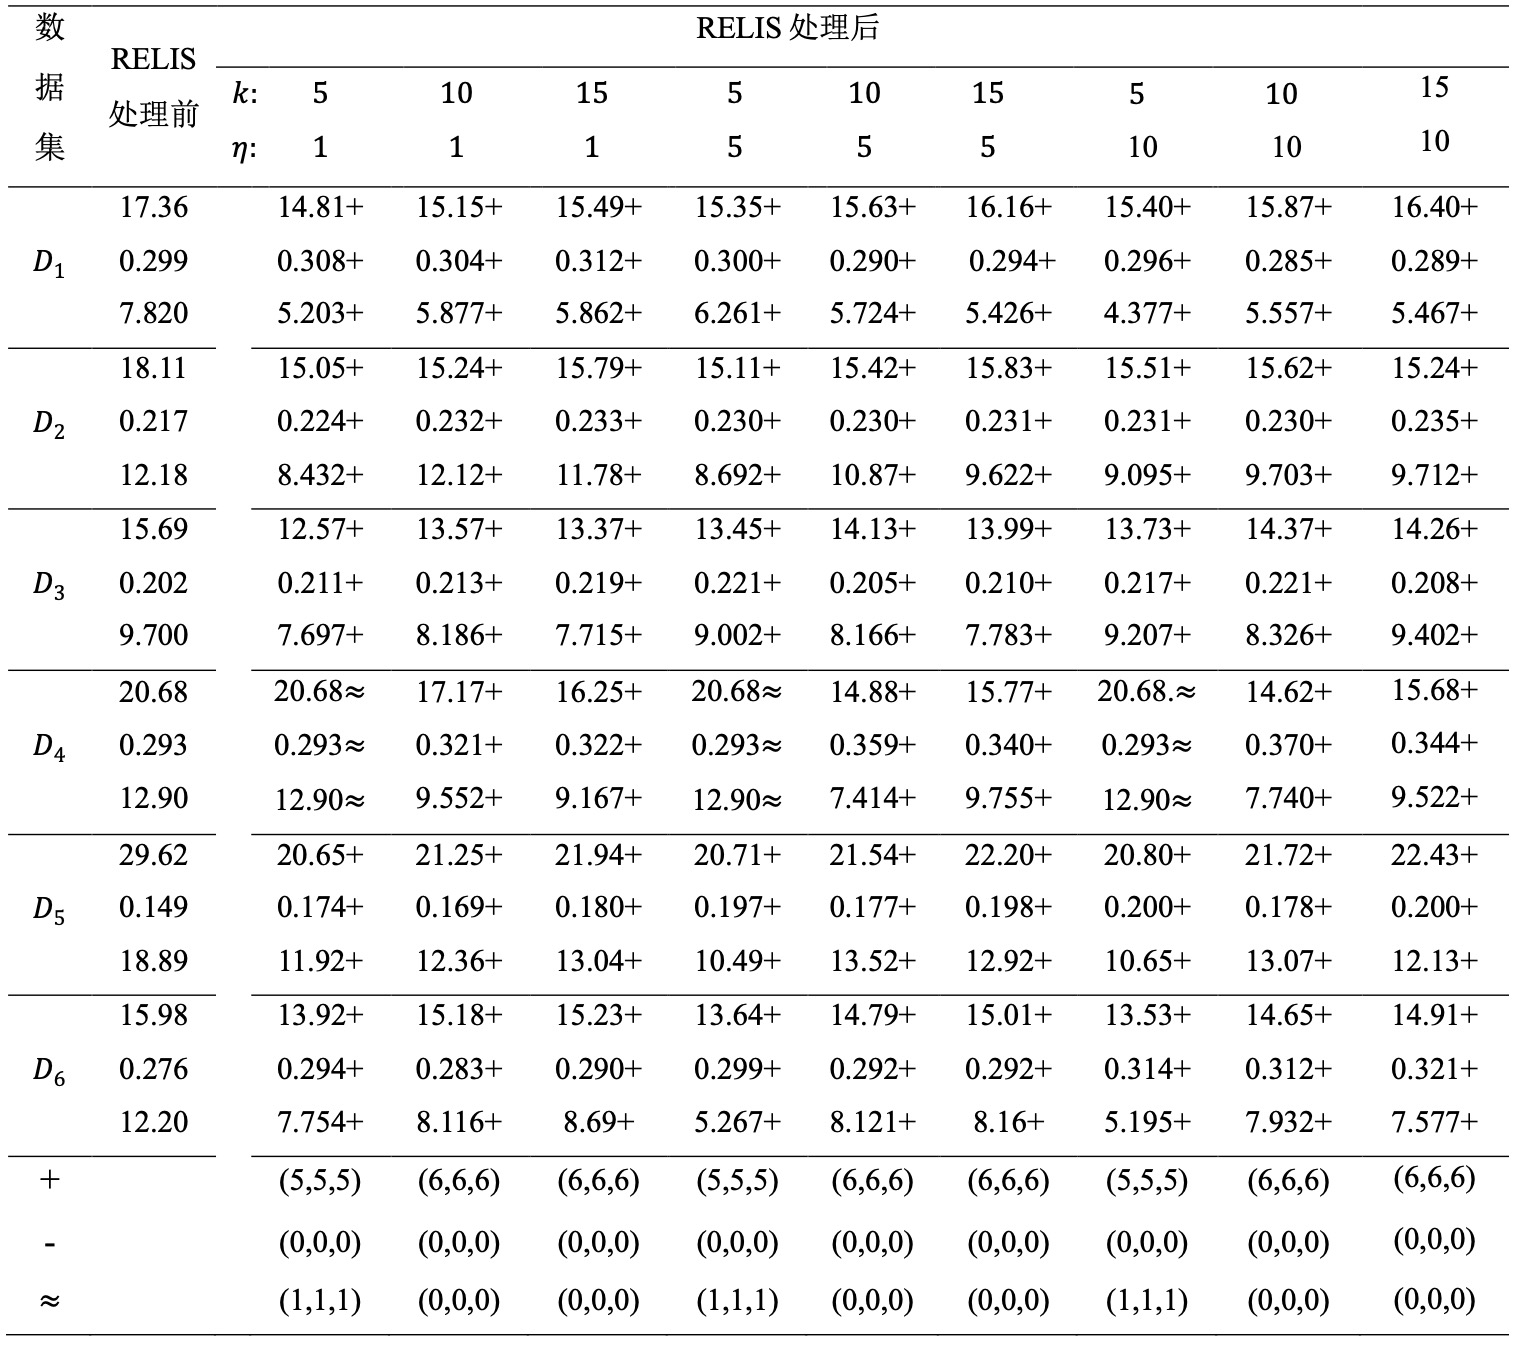
\includegraphics[width=1.0\textwidth]{模拟实验结果.jpg}
		\label{tab3}
	\end{figure}

	根据实验结果可知,大多数情况下,原始数据集经过RELIS方法处理后各项指标均能得到优化。注意到数据集 $D_4$,当超参数 $k=5,\eta=1,5,10$时,各项指标未发生改变。这主要是因为随着特征维数的增加,大多数簇的样本在特征空间中变得过于稀疏。
	在KNN优化阶段,所有样本被合并到一个簇中,跳过了RELIS的后续处理阶段,因此并未合成新的样本。然而,随着超参数k的值增加,这一问题得以解决。

	相较于 $\eta$,超参数k对于优化结果具有更强的敏感性,这一点会在后续的实验中得到验证。在超参数k的取值合适的情况下,随着 $\eta$的增加,会进一步提升各项指标的优化效果。

	实验结果还表明,即使对于大方差噪声占比较高的情况下(见数据集$D_5$),RELIS依旧表现出良好的优化效果,这说明该方法可以处理更复杂的噪声,并具有良好的鲁棒性。此外,即使面对样本量较少的数据集$D_6$以及具有厚尾特征分布的数据集 $D_4$,RELIS方法也能表现出良好的优化效果。


	\subsection{超参数分析}

	为了更全面地分析不同超参数下RELIS对原始数据集的优化效果,本文计算了优化前的指标与经过RELIS方法优化后的指标差值,以便更直观分析其在不同超参数组合下的优化效果,结果见图3。

	\begin{figure}[t!]
		\centering
		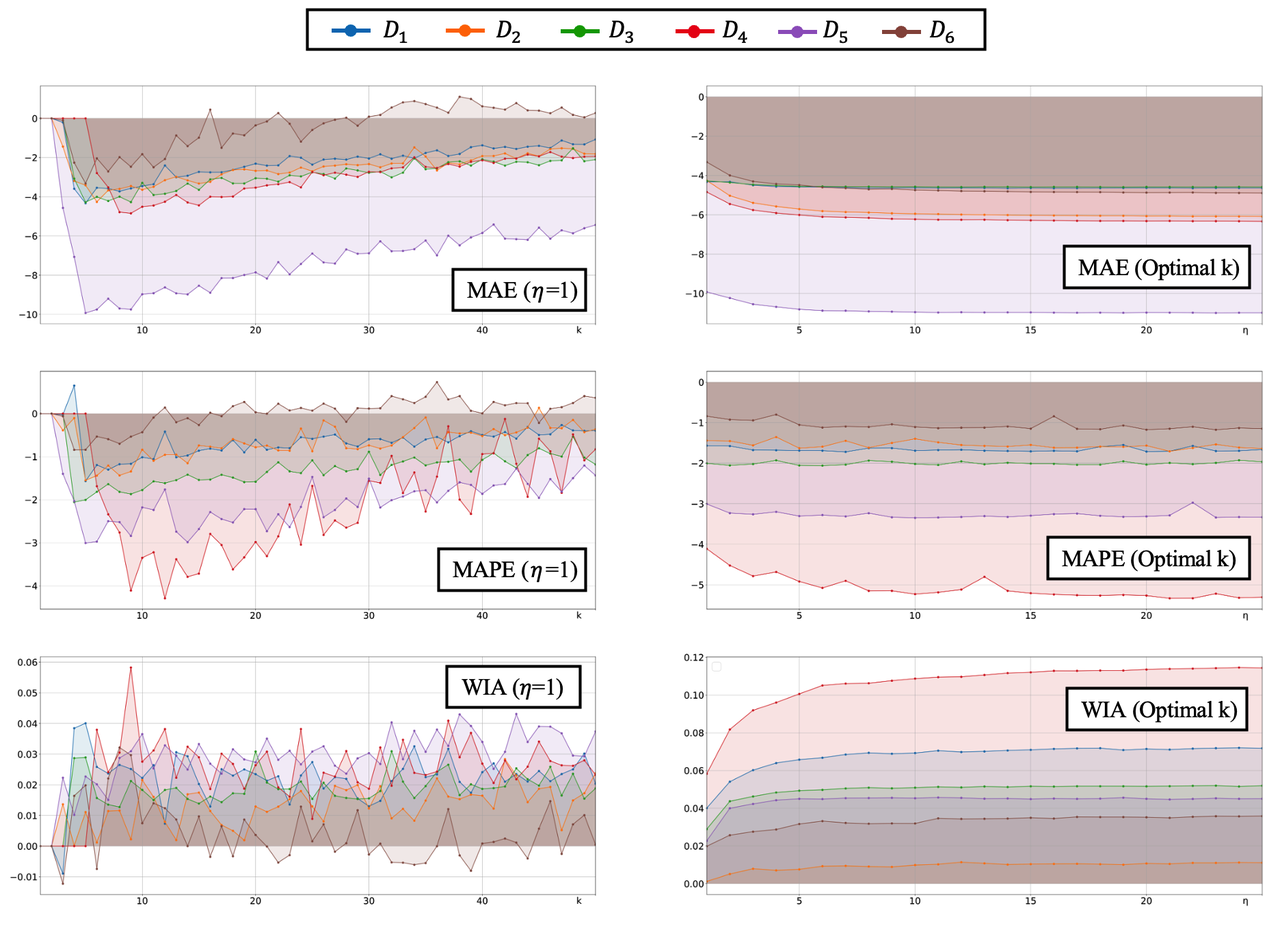
\includegraphics[width=1.0\textwidth]{不同超参数下RELIS方法优化效果.png}
		\caption{不同超参数下RELIS方法优化效果}
		\label{fig5}
	\end{figure}
	在图3中,左边三幅图展示了当超参数 $\eta=1$时,不同超参数 $k$值下三个指标的优化效果;右边三幅图展示了超参数$k$取MAE指标最优情况时,不同超参数$\eta$下RELIS方法的优化效果。相比MAE以及WIA,MAPE具有更大的波动性。
	这主要是因为RELIS合成了更多真实值接近0的样本,而MAPE指标对于真实值接近0的样本异常敏感,这在数据集$D_2$中表现更加明显;在不同超参数$k$下,RELIS方法对于MAE以及MAPE的优化效果呈现U形,WIA则会在一个稳定的范围小幅度波动;相比于超参数$k$,
	超参数$\eta$对于优化效果的影响更加稳定。在大多数情况下,随着超参数 $\eta$的增加,各项指标的优化效果会得到进一步提升;通过MAPE指标的性质可以看出,经过RELIS方法优化后,噪声较大的样本占比明显下降,噪声较小的样本占比提升。

	\section{实例分析}
		
	\subsection{数据集介绍}
	本节使用四个实例数据集去检验RELIS方法对于预测模型的优化表现\cite{bib27,bib28,bib29,bib30},具体如下:
	
	“Bike Sharing Demand”数据集是专为预测城市自行车共享系统中的租赁需求而设计的,其数据源自华盛顿特区的Capital Bikeshare 程序,覆盖2011年至2012年期间的细致使用记录。这个数据集详细记录了每个小时的租赁活动,同时附有天气情况、日期和时间等相关信息。
	具体而言,数据集涵盖了季节变化、是否为假期、是否为工作日以及四种不同的天气情况,从晴朗到大雨或雪。此外,每个时间点的温度、湿度、风速等气象信息也被包括在内,旨在帮助参赛者通过这些信息预测每小时的自行车租赁数量。
	
	“Air Quality”数据集集中于环境监测,提供了详尽的空气质量指标记录,旨在评估和预测各地的空气质量状况。该数据集包含从多个监测站收集的空气污染浓度数据,如二氧化氮($NO_2$)、颗粒物($PM10$和$PM2.5$)、一氧化碳($CO$)、臭氧($O_3$)等,这些数据通常以小时或日为单位记录。
	除了污染物浓度,数据集还包括温度、湿度、气压等气象条件信息。
	
	“Facebook Metrics”数据集关联于2014年某知名化妆品牌Facebook页面发布的帖子,该数据集包含Moro等人(2016年)发布帖子之前已知的7个特征和用于评估帖子影响的12个特征,以及提供了每个帖子获得用户点赞的数量。
	
	“Forest Fires”数据集是由葡萄牙的Montesinho自然公园内的森林火灾记录构成的,这个数据集广泛用于研究和分析森林火灾的发生情况与多种可能的影响因素之间的关系。该数据集包含了从1998到2003年间,关于森林火灾的517条记录,涵盖了如气象条件(包括温度、湿度、风速和降雨量等)以及空间数据(如火灾发生的月份和日期、火灾发生的坐标位置等)。
	这些特征被用于预测特定条件下森林火灾的燃烧面积,是研究森林火灾行为、评估火灾风险以及制定预防措施的中药资源。通过分析这个数据集,研究人员可以构建和测试模型,以预测和理解在特定气候和地理条件下森林火灾的行为,从而有助于森林管理和火灾预防工作。
		
	\subsection{优化效果分析}
	\begin{figure}[t!]
		\centering
		\caption*{表4:  实例数据集实验结果}
		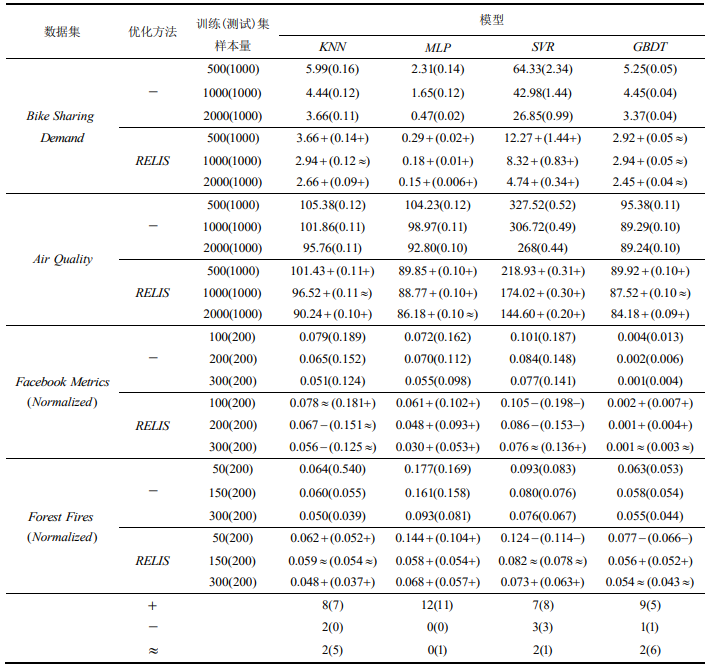
\includegraphics[width=1.0\textwidth]{模拟实验结果.png}
		\label{tab3}
	\end{figure}

	对每个数据集,随机选择不同数量规模的样本,划分为训练集与测试集。本文对训练集数据使用RELIS方法处理,随后训练模型,并在测试集上检验模型的预测效果。
	对于每一组实验依旧重复25次,并取平均值作为实验结果。之后进行威尔克森符号秩检验,以检验RELIS方法是否对模型的预测性能具有优化效果。选取的机器学习模型包括:K最近邻(KNN),多层感知机(MLP),梯度提升决策树(GBDT)以及支持向量回归机(SVR)。对于需要超参数调优的模型如GBDT、KNN,多次选择不同的超参数并取最好的实验结果,SVR的核函数选择径向基函数(RBF)。此外,本文剔除了无法直接使用的数据特征,如Bike Sharing Demand 数据集中的“Datetime”,Forest Fires 数据集中的“Month”等。
	本文选用MAE以及MAPE两个指标度量RELIS方法对于预测模型泛化能力的优化效果,原始训练集使用RELIS优化前后各个模型的预测表现如表4所示,其中括号内的数据为MAPE指标的实验计算结果。
	通过表4可知:
	

	(1).大多数情况下RELIS方法都显著提升了模型的预测效果,对于所有的模型RELIS都表现出了良好的适应能力;

	(2).即使针对小样本数据集以及标准化处理后的数据集,如“Facebook Metrics”,RELIS依旧可以显著提升模型的预测能力;

	(3).该部分实验并未删除掉非连续型变量的特征,这一点违背了RELIS方法变量连续的假设,并且针对样本量较少的情况,很难满足RELIS方法线性拟合函数误差趋向于0的假设。由此可见,即使违背了RELIS方法的假设,RELIS方法依旧可以对模型的预测效果显著优化,这也从另一方面体现了该方法的鲁棒性。


	\section{结论}
	本文基于特征子空间插值的思想提出了 一种创新的对于含噪数据集优化的数据合成方法,命名为RELIS方法。该方法可以在保证不损害样本原始信息的前提下,
	合成大量具有较小误差的样本,从而提升机器学习模型的泛化能力。本文通过生成含有复杂且未知噪声的数据集对RELIS方面进行了全面的模拟研究,实验结果
	表明RELIS方法对于含噪数据集具有显著的优化效果。在实例数据中,本文将经过RELIS优化后的样本用于机器学习实际的预测场景中,实验结果表明该方法可以显著提升模型的泛化能力。

	\bibliography{ref}
	\bibliographystyle{IEEEtran}
	\newpage
	\section*{附录}
	\noindent\textbf{定理1证明:}由于 $\varepsilon^\prime\rightarrow0$, 根据公式$(5)$,可得: 
	$$y^{s,s+1}=g_{s,s+1}(x^{s,s+1})+\varepsilon.$$
	将公式 $(7)$转化为:
	$$\bar{S}(x^s,x^{s+1})=\frac{\int_{x^s}^{x^{s+1}}|g(x)-l(x)|  dx}{|x^{s+1}-x^s|}.$$
	根据迭代期望法则$(LIE)$:
	$$\begin{aligned}
		\mathbb{E}(\bar{S}(x^s,x^{s+1}))&=\mathbb{E}(\bar{S}(x^s,x^{s+1})|\varepsilon^s\cdot\varepsilon^{s+1}<0)P(\varepsilon^s\cdot\varepsilon^{s+1}<0) \\
		&\quad\; +\mathbb{E}(\bar{S}(x^s,x^{s+1})|\varepsilon^s\cdot\varepsilon^{s+1}\ge0)P(\varepsilon^s\cdot\varepsilon^{s+1}\ge0)
		\end{aligned}$$
	我们可以利用基本的几何面积计算来简化 $\bar{S}(x^s,x^{s+1})$。如果$\varepsilon^s\cdot\varepsilon^{s+1}<0$,那么$\exists{x'}\in(x^s,x^{s+1})$,使得 $g(x')=l(x')$。由此得出:
	$$\mathbb{E}(\bar{S}(x^s,x^{s+1})|\varepsilon^s\cdot\varepsilon^{s+1}<0)=\frac{\mathbb{E}(|\varepsilon^s|)\cdot|x^s-x'|+\mathbb{E}(|\varepsilon^{s+1}|)\cdot|x^{s+1}-x'|}{2|x^{s+1}-x^s|}.$$
	如果$\varepsilon^s\cdot\varepsilon^{s+1}\ge0$,则有:
	$$\begin{aligned}
    \mathbb{E}(\bar{S}(x^s,x^{s+1})|\varepsilon^s\cdot\varepsilon^{s+1}\ge0)&=\frac{\mathbb{E}(|\varepsilon^s|+|\varepsilon^{s+1}|)\cdot|x^{s+1}-x^{s}|}{2|x^{s+1}-x^s|}\\&=\frac{\mathbb{E}(|\varepsilon^s|+|\varepsilon^{s+1}|)}{2}.
    \end{aligned}$$
	将其代入原始公式中,可以推导出:
	$$\begin{aligned}
		\mathbb{E}({\bar{S}(x^{s}, x^{(s+1)})})&=
		\frac{{\mathbb{E}(|\varepsilon^s|)\cdot|x^s-x'|+\mathbb{E}(|\varepsilon^{s+1}|)\cdot|x^{s+1}-x'|}}{2|x^{s+1}-x^s|}P(\varepsilon^s\cdot\varepsilon^{s+1}<0)\\
		&\;\quad+\frac{\mathbb{E}(|\varepsilon^s|+|\varepsilon^{s+1}|)}{2}P(\varepsilon^s\cdot\varepsilon^{s+1}\ge0).
		\end{aligned}$$
	注意到$P(\varepsilon^s\cdot\varepsilon^{s+1}<0)+P(\varepsilon^s\cdot\varepsilon^{s+1}\ge0)=1$,并且:
	$$\begin{aligned}
		\frac{{\mathbb{E}(|\varepsilon^s|)\cdot|x^s-x'|+\mathbb{E}(|\varepsilon^{s+1}|)\cdot|x^{s+1}-x'|}}{2|x^{s+1}-x^s|}&=
    	\frac{{\mathbb{E}(|\varepsilon^s|)\cdot|\frac{x^s-x'}{x^{s+1}-x^s}|+\mathbb{E}(|\varepsilon^{s+1}|)\cdot|\frac{x^{s+1}-x'}{x^{s+1}-x^s}|}}{2}\\
    	&<\frac{{\mathbb{E}(|\varepsilon^s|)+\mathbb{E}(|\varepsilon^{s+1}|)}}{2},
		\end{aligned}$$
		得证:
		 $$\mathbb{E} (\bar{S}(x^s,x^{s+1}))< \mathbb{E}(\frac{|\varepsilon^s|+|\varepsilon^{s+1}|}{2}).$$

	\noindent\textbf{定理2证明:}如果$\varepsilon^s\cdot\varepsilon^{s+1}<0$时,$\exists x'\in(x^s,x^{s+1})$,使得
	$g(x')=l(x')$。由此得出:
	$$\begin{aligned}
		\bar{
		S}(x^s,x^{s+1})&=\frac{|\varepsilon^{s}|\cdot|x^{s}-x'|+|\varepsilon^{s+1}|\cdot|x^{s+1}-x'|}{2|x^s-x^{s+1}|}\\
		&=\frac{|\varepsilon^{s}|\cdot|\frac{x^s-x'}{x^{s}-x^{s+1}}|+|\varepsilon^{s+1}|\cdot|\frac{x^{s+1}-x'}{x^{s}-x^{s+1}}|}{2}.
		\end{aligned}$$
	基于相似三角形的性质,我们可以推断:
	$$|\frac{x^s-x'}{x^{s}-x^{s+1}}|=|\frac{\varepsilon^s}{\varepsilon^s-\varepsilon^{s+1}}|,$$
	$$|\frac{x^{s+1}-x'}{x^{s}-x^{s+1}}|=|\frac{\varepsilon^{s+1}}{\varepsilon^s-\varepsilon^{s+1}}|.$$
	代入原式,可以推导出:
	$$\begin{aligned}
		\bar{
		S}(x^s,x^{s+1})&=
		\frac{|\frac{\varepsilon^s}{\varepsilon^s-\varepsilon^{s+1}}|\cdot |\varepsilon^{s}|+|\frac{\varepsilon^{s+1}}{\varepsilon^s-\varepsilon^{s+1}}|\cdot|\varepsilon^{s+1}|}{2}.
		\end{aligned}$$
	如果$\varepsilon^s\cdot\varepsilon^{s+1}\ge0$时,那么:
	$$\begin{aligned}
		\bar{
		S}(x^s,x^{s+1})&=\frac{(|\varepsilon^s|+|\varepsilon^{s+1}|)\cdot|x^{s+1}-x^{s}|}{2|x^{s+1}-x^{s}|}\\&=
		\frac{|\varepsilon^s|+|\varepsilon^{s+1}|}{2}.
		\end{aligned}$$
	\noindent\textbf{定理3证明:}由于线性拟合误差$\varepsilon^\prime\rightarrow0$,根据公式(5)可得:
	$$y^{s,s+1}=g_{s,s+1}(\boldsymbol{x}^{s,s+1})+\varepsilon.$$
	根据公式(11)和(12):
	$$\begin{aligned}
		\varepsilon^{s,s+1}_{(d)}&=y_{(d)}^{s,s+1}-f(\boldsymbol{x}_{(d)}^{s,s+1})\\&=
		y^s+d\dfrac{y^{s+1}-y^{s}}{\left\lceil \frac{n\eta}{\text{dist}_{\text{sum}}}\text{dist}(\boldsymbol{x}^s,\boldsymbol{x}^{s+1})\right\rceil+1}-f{(\boldsymbol{x}^s+d\dfrac{\boldsymbol{x}^{s+1}-\boldsymbol{x}^{s}}{\left\lceil \frac{n\eta}{\text{dist}_{\text{sum}}}\text{dist}(\boldsymbol{x}^s,\boldsymbol{x}^{s+1})\right\rceil+1})}\\&=
		y^s+d\dfrac{y^{s+1}-y^{s}}{\left\lceil \frac{n\eta}{\text{dist}_{\text{sum}}}\text{dist}(\boldsymbol{x}^s,\boldsymbol{x}^{s+1})\right\rceil+1}-g{(\boldsymbol{x}^s+d\dfrac{\boldsymbol{x}^{s+1}-\boldsymbol{x}^{s}}{\left\lceil \frac{n\eta}{\text{dist}_{\text{sum}}}\text{dist}(\boldsymbol{x}^s,\boldsymbol{x}^{s+1})\right\rceil+1})}
		\end{aligned}$$
	令$\dfrac{d}{\left\lceil \frac{n\eta}{\text{dist}_{\text{sum}}}\text{dist}(\boldsymbol{x}^s,\boldsymbol{x}^{s+1})\right\rceil+1}=m$,可得:
	$$\begin{aligned}
		\varepsilon^{s,s+1}_{(d)}&=y^s-g(\boldsymbol{x}^s)+m\cdot(y^{s+1}-g(\boldsymbol{x}^{s+1})-y^s+g(\boldsymbol{x}^{s}))\\&=
		\varepsilon^s+m\cdot(\varepsilon^{s+1}-\varepsilon^s)\\&=
		(1-m)\cdot\varepsilon^s+m\cdot\varepsilon^{s+1}.
		\end{aligned}.$$
	由于$0<m<1$,有:\\
	$$\begin{aligned}
		&\mathbb{E}(\frac{\textstyle\sum_{d=1}^{{\left\lceil \frac{n\eta }{\text{dist}_{\text{sum}}}\text{dist}(\boldsymbol{x}^s,\boldsymbol{x}^{s+1})\right\rceil}}{|\varepsilon^{s,s+1}_{(d)}|}}{\left\lceil \frac{n\eta }{\text{dist}_{\text{sum}}}\text{dist}(\boldsymbol{x}^s,\boldsymbol{x}^{s+1})\right\rceil})\\&=
		\frac{\textstyle\sum_{d=1}^{{\left\lceil \frac{n\eta }{\text{dist}_{\text{sum}}}\text{dist}(\boldsymbol{x}^s,\boldsymbol{x}^{s+1})\right\rceil}}{
		\mathbb{E}|\varepsilon^{s,s+1}_{(d)}|}}{\left\lceil \frac{n\eta }{\text{dist}_{\text{sum}}}\text{dist}(\boldsymbol{x}^s,\boldsymbol{x}^{s+1})\right\rceil}\\&=
		\frac{\textstyle\sum_{d=1}^{{\left\lceil \frac{n\eta }{\text{dist}_{\text{sum}}}\text{dist}(\boldsymbol{x}^s,\boldsymbol{x}^{s+1})\right\rceil}}{
		\mathbb{E}|(1-m)\cdot\varepsilon^s+m\cdot\varepsilon^{s+1}|}}{\left\lceil \frac{n\eta }{\text{dist}_{\text{sum}}}\text{dist}(\boldsymbol{x}^s,\boldsymbol{x}^{s+1})\right\rceil}\\&<
		\frac{\textstyle\sum_{d=1}^{{\left\lceil \frac{n\eta }{\text{dist}_{\text{sum}}}\text{dist}(\boldsymbol{x}^s,\boldsymbol{x}^{s+1})\right\rceil}}{
		\mathbb{E}(|(1-m)\cdot\varepsilon^s|+|m\cdot\varepsilon^{s+1}|)}}{\left\lceil \frac{n\eta }{\text{dist}_{\text{sum}}}\text{dist}(\boldsymbol{x}^s,\boldsymbol{x}^{s+1})\right\rceil}\\&=
		\frac{\mathbb{E}|\varepsilon^s|\textstyle\sum_{d=1}^{{\left\lceil \frac{n\eta }{\text{dist}_{\text{sum}}}\text{dist}(\boldsymbol{x}^s,\boldsymbol{x}^{s+1})\right\rceil}}{
		(1-m)+\mathbb{E}|\varepsilon^{s+1}|}\textstyle\sum_{d=1}^{\left\lceil \frac{n\eta}{\text{dist}_{\text{sum}}}\text{dist}(\boldsymbol{x}^s,\boldsymbol{x}^{s+1})\right\rceil}m}{\left\lceil \frac{n\eta }{\text{dist}_{\text{sum}}}\text{dist}(\boldsymbol{x}^s,\boldsymbol{x}^{s+1})\right\rceil}\\
		&=
		\frac{\mathbb{E}|\varepsilon^s|\textstyle\sum_{d=1}^{{\left\lceil \frac{n\eta }{\text{dist}_{\text{sum}}}\text{dist}(\boldsymbol{x}^s,\boldsymbol{x}^{s+1})\right\rceil}}{
		(1-m)}}{\left\lceil \frac{n\eta }{\text{dist}_{\text{sum}}}\text{dist}(\boldsymbol{x}^s,\boldsymbol{x}^{s+1})\right\rceil} + \frac{{\mathbb{E}|\varepsilon^{s+1}|}\textstyle\sum_{d=1}^{\left\lceil \frac{n\eta}{\text{dist}_{\text{sum}}}\text{dist}(\boldsymbol{x}^s,\boldsymbol{x}^{s+1})\right\rceil}m}{\left\lceil \frac{n\eta }{\text{dist}_{\text{sum}}}\text{dist}(\boldsymbol{x}^s,\boldsymbol{x}^{s+1})\right\rceil}
		\\
		&=\mathbb{E}(\frac{|\varepsilon^s|+|\varepsilon^{s+1}|}{2}).
		\end{aligned}$$
	综上,得证。

	% \newpage

	% {\Large\textbf{for Recurrent Event Data} \par}
	% \vspace{12pt}
	
	% {\large{\begin{center}Lu Min;Lou Zhilong;Cai Yitao;Wang Han;Du Yukun;moumoumou;Li Yao\end{center}}\par }
	% \vspace{5pt}
	% {\begin{center}({\small Nanjing Audit University, Nanjing 210000} )\end{center}}\par
	% \vspace{7pt}
	
	% {\begin{center}({\small E-mail: })\end{center}}\par
	
	
	\


	
	% \hskip1.54cm estimating equation

	% \noindent{\bf MR(2000) Subject Classification}\quad 62G05; 62N015
	
	% \noindent{\bf Chinese Library Classification}\quad O212.7



\end{document}% 结束文档编辑,后面写啥都编译不出来

